\subsection{Insertion Sort}\label{subsec:insertion-sort-laufzeit}

\subsection{Quick Sort}\label{subsec:quick-sort-laufzeit}

\subsubsection{Pivot Methoden}

\paragraph{Erste Implementation}
Bei der ersten Implementation vom Quicksort Algorithmus ist bei der
Verwendung der Pivot-Methoden \(right\) und \(median\)  eine deutlich längere
Laufzeit aufgefallen (siehe Abbildung~\ref{fig:qsort-first-impl}).
Gleichzeit ist die Laufzeit von der \(middle\) Pivot Methode besser, obwohl
die Erwartung dieser schlechter ist:
Diese muss eineinhalb mal -- einmal zum finden der Länge \(l\) komplett, danach
bis zum \(l/2\) Element -- durchlaufen werden.
Die Pivot Methode \(right\) muss nur einmal bis zum Ende der Liste laufen.

\begin{figure}[hbt]
    \caption{Vergleich der Pivot Methoden 1}
    \centering
    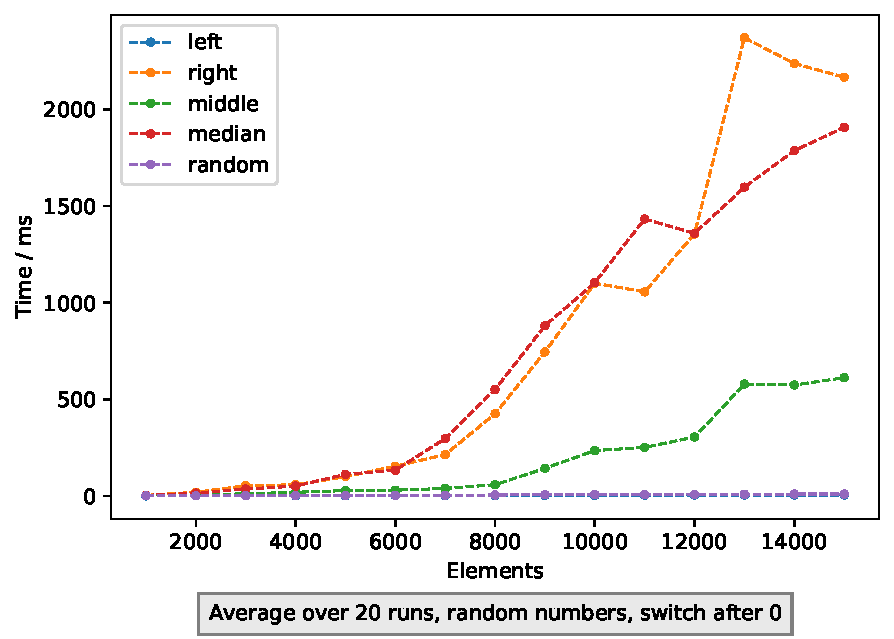
\includegraphics[width = 8cm]
    {../out/pivotMethods_Implementation1.pdf}\label{fig:qsort-first-impl}
\end{figure}

Unsere erste Vermutung war, dass unsere Methoden, die in einem
Durchlauf die Länge und gleichzeitig dass Pivot-Element ermitteln dafür
verantwortlich sein könnten.
In der Methoden zum Finden des letzten Elementes, die auch von der median
Pivot Methode verwendet wird, benutzten wir Pattern Matching, um zwischen dem
Letzten und vorletztem Element zu unterscheiden.
Dabei muss allerdings jeweils vorausgeschaut werden, was die schlechte
Performance erklären könnte.

Somit die Vermutung, dass man die Performance verbessern kann, indem man
zunächst die Länge der Liste ermittelt und anschließend diese zum Finden des
n-ten Elements ein zweites mal durchläuft.

\paragraph{Zweite Implementation}

In der zweiten Implementation wurden die Ermittlung des Pivots und das Finden
der Länge der Liste getrennt.
Das letzte Elements wurde nun ermittelt, indem zunächst
die Länge \(l\) der Liste berechnet, anschließend mithilfe dieser zum
\(l-1\) -ten Element gelaufen wird.
\begin{figure}[hbt]
    \centering
    \caption{Zweite Implementation}
    \subfloat[median]{
    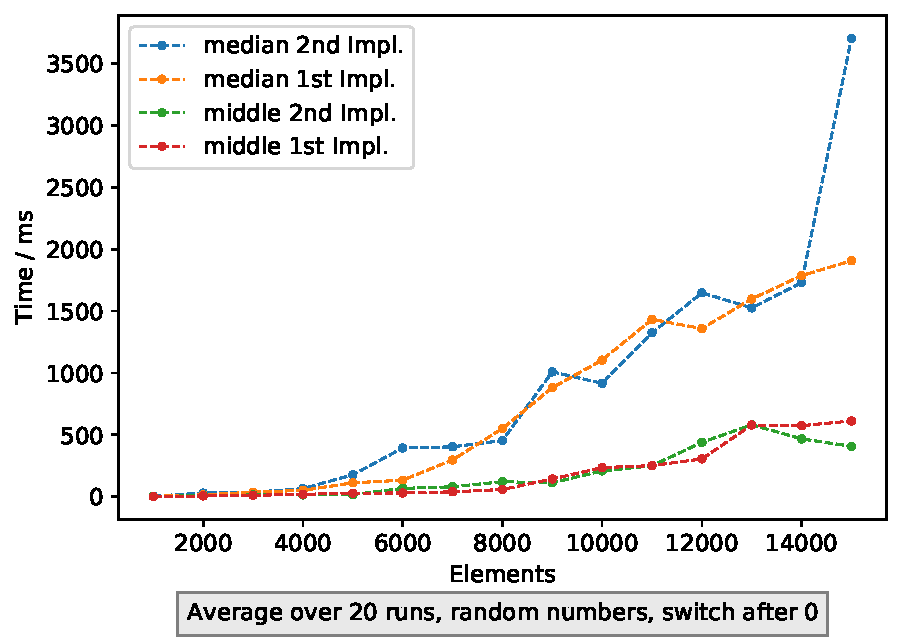
\includegraphics[width = 0.47\textwidth]
    {../out/pivotMethods_Implementation2b.pdf}\label{fig:qsort-impl2b} }
    \hfill
    \subfloat[right]{
    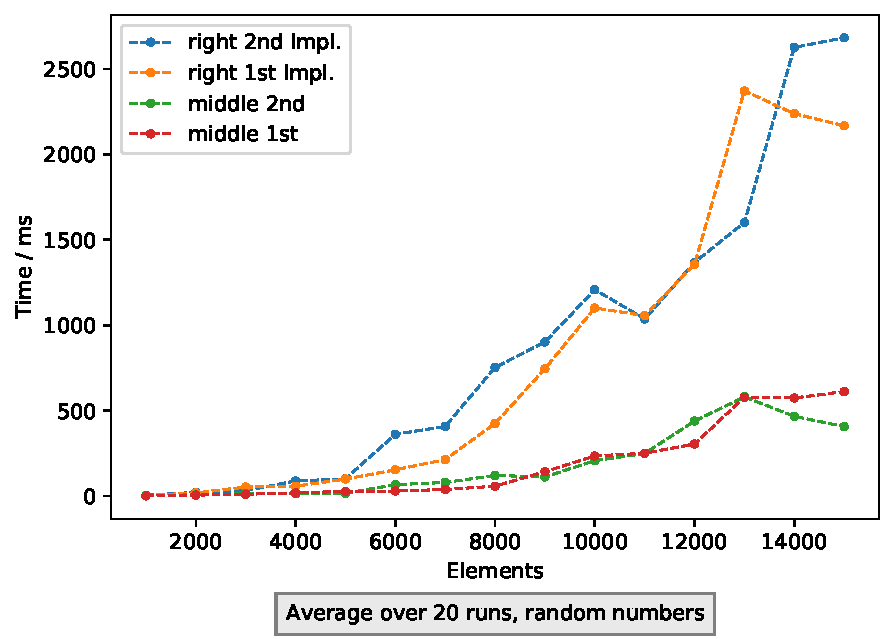
\includegraphics[width = 0.47\textwidth]
    {../out/pivotMethods_Implementation2a.pdf}\label{fig:qsort-impl2a} }
\end{figure}


In Abbildung~\ref{fig:qsort-impl2b} und~\ref{fig:qsort-impl2a} sind jeweils die
Ergebnisse der Laufzeitmessung der zweiten Implementation von \(median\) und
\(right\) zu sehen.
Damit systematische Unterschiede zwischen den beiden Kompilationen
ausgeschlossen sind, ist zusätzlich die gleiche Implementation, von \(middle\)
dargestellt.
Bei beiden überarbeiteten Implementationen ist keine Besserung der Laufzeit zu
erkennen, was darauf schließen lässt, dass das in der ersten Implementation
verwendete Pattern Matching nicht der Grund der schlechten Performance war.

\FloatBarrier

\subsection{Heap Sort}\label{subsec:heap-sort-laufzeit}
